\chapter{Paper-based semantic speech editing}\label{sec:paper}

In Chapter~\ref{sec:ethno}, we found that two of the three radio production teams we observed used paper as part of
their current production workflow.  We also saw that all of the radio producers we observed used transcripts to help
them navigate and structure their content.  In Chapter~\ref{sec:screen}, we saw that some radio producers found their
work environment noisy and distracting, and did not like working with screens for extended periods.  One of the study
participants chose to print their transcripts as they found the production process easier to achieve on paper than
directly on screen.


Working on paper offers a number of advantages over working on screens.  Paper is lightweight, portable and does not
require any power, which allows users to work almost anywhere.  It is not back-lit, so is easier on the eyes.  It can
be navigated quickly, annotated freely whilst reading, and individual pages can be laid out and easily compared.  Its
physical low-tech nature also means that it is intuitive, robust, durable and does not crash or lose data.  Reading
from paper rather than a screen has been found to improve comprehension \citep{Mangen2013}, recollection
\citep{Singer2017}, sense of structure and cross-referencing \citep{OHara1997} and to be faster \citep{Kurniawan2001}.

Radio producers can use paper to make hand-written annotations to help them structure their program and make editorial
decisions.  However, printing a document breaks the link to its digital source, so is normally a one-way process in
which any information that is changed/added is not fed back.  For example, when a producer uses the paper transcript to
decide which parts of the audio they want to use in their programme, they must use a digital audio workstation (DAW) to
manually execute those editorial decisions, which is a tedious and slow process.  Creating a ``digital bridge'' between
paper and its digital source may allow us to combine the advantages of paper and digital workflows.


In this chapter, we describe the design, development and evaluation of \textit{Paper\-Clip} --- a novel system for editing
speech recordings directly on a printed transcript using a digital pen.  In Section~\ref{sec:paper-background} we
review previous approaches to semantic speech editing and natural annotation of digital content. In
Section~\ref{sec:paper-requirements} we describe our first study in which we worked with radio producers to design the
layout of our system. In Section~\ref{sec:paper-design} we describe the design of PaperClip, which we developed in
collaboration with a digital pen manufacturer. In Section~\ref{sec:paper-method} we explain the methodology of our
second study in which radio producers edited content for their programmes using PaperClip, a screen interface and a
normal printed transcript.  We present the results in Section~\ref{sec:paper-results} which compares the strengths of
the digital pen and screen interfaces, and shows how the accuracy of the transcript and listening affect the editing
process.  We discuss these results in Section~\ref{sec:paper-discussion} and present our conclusions in
Section~\ref{sec:paper-conclusion}.


\section{Background}\label{sec:paper-background}


Our system combines semantic editing of speech with natural annotation of digital content. As we saw in
Section~\ref{sec:background-semantic-editing}, previous semantic speech editing systems have all used screen
interfaces. We identified three alternative types of interfaces that could be used to edit digital content:
barcodes,
digital pens,
and digital ink.
In this section, we explore each of these approaches and their applications.

\subsection{Barcodes}
Barcodes printed on paper transcripts have been explored as a method of navigating video recordings by using a device
to scan the barcode and play the video from that position. \textit{Video Paper} \citep{Hull2003} was a system that
printed video keyframes and barcodes down the side of a paper transcript. Each barcode linked to a position in a video,
which was downloaded from a database and played on the scanning device. \textit{Books with Voices} \citep{Klemmer2003}
was a similar system that tested this approach on oral historians who found it effective for assisting a transcript
editing task. \citet{Erol2007} went a step further by embedding the video data in the barcode, removing
the need for a database.  \textit{HotPaper} \citep{Erol2008} removed the need for barcodes by using a camera to measure
the whitespace between words and matching that to unique patterns in the text.

Barcode-based systems provide a link between text and media. They use real paper, can be annotated freely, are easy to
generate and are robust to photocopying.  However, they do not provide a convenient method of capturing annotations. It
would be possible to use a handheld device to capture annotations and link them to a particular barcode.  However, this
would require the annotations to be entered into a handheld device, rather that just written on the paper.
Additionally, the size of barcodes means that they cannot be used for each word, which affects the precision of the
system.

\subsection{Digital pens}

A digital pen looks and functions as a normal pen, but includes an on-board infrared camera that tracks the position of
the pen while it writes on paper. Digital pens must be used in combination with paper that has a unique non-repeating
dot pattern printed onto it using a standard colour laser printer.  By reading this pattern, the pen can calculate
exactly where it is when touching the page. The pen records its position up to 100 times a second.  Depending on the
pen and software, this information can either be streamed live via Bluetooth, or downloaded as a batch onto a computer.
The digital pens that use this patented technology \citep{Fahraeus2003} are exclusively manufactured and licensed by
Anoto Group. As such, this technology is commonly referred to as the \textit{Anoto dot pattern}.

\textit{ChronoVis} \citep{Fouse2011} was a note-taking system that used the Anoto pattern for recording synchronised
hand-written notes during playback of a video. An accompanying screen interface allowed users to click on the digital
display of the handwritten notes to navigate to that position in the video. %
\citet{Weibel2012} conducted a longitudinal study of ChronoViz for use in observational research. The results show that
notes became a mixture of linear notes and symbolic representations.  Asterisks, stars, lines and simple shapes were
used as bookmarks for later referral, or for counting events.  The flexibility of freehand notes also enabled use of
arrows in various contexts, such as to indicate direction and actions.

\textit{PADD} \citep{Guimbretiere2003} was a concept for a system of editing documents that used the Anoto pattern to
allow users to move from digital to paper and back again.  \textit{ProofRite} \citep{Conroy2004} was the first full
implementation of a PADD system, which overlaid annotations made on paper into a word processor. The annotations are 
anchored to the text, such that they ``reflow'' when the text is moved.  Through informal feedback, users suggested
that their annotations should translate into actions such as delete.  \textit{PaperProof} \citep{Weibel2008}
interpreted edit annotations and automatically applied them to the document.  Gestures for delete, insert, replace,
move and annotate were translated into modifications in a word processor, and intelligent character recognition was
used to digitise any hand-written text. The interpretation of annotations allows for a two-way interaction between the
digital and paper representations. We could not find any user studies of the PaperProof system.




\subsection{Digital ink}
\textit{Digital ink} refers to technology that digitally captures and responds to the movements of a pen, such as a
stylus.  Typically, digital ink systems use a device with a backlit screen and a touch-sensitive interface like a
tablet PC.  Several systems have experimented with using a stylus with interactive sliders to provide advanced control
for navigating video content. Examples include \textit{LEAN} \citep{Ramos2003}, \textit{Zlider} \citep{Ramos2005} and
\textit{MobileZoomSlider/ScrollWheel} \citep{Huerst2008}. However, these systems are limited to the navigation of
content, without changing or labelling it.  As we will see in this section, digital ink interfaces can also be used to
annotate and edit media.

\textit{Marquee} \citep{Weher1994} synchronised handwritten notes with a live video recording by using a horizontal
line gesture to mark a timestamp.  \textit{Dynomite} \citep{Wilcox1997} synchronised handwritten notes to a live audio
recording, and allowed the user to categorise their annotations using keywords, and to highlight regions of audio using
a button.  In the evaluations of each of their systems, \citet{Weher1994} and \citet{Wilcox1997} both found that users
took fewer notes when using the digital ink system, and that they wanted to go back and use the audio/video to improve
the notes afterwards.



\textit{Videotater} \citep{Diakopoulos2006} was another digital ink interface for segmenting and annotating
pre-recorded video clips. A vertical line gesture on a video timeline split the video into a clip, which could be
labelled with handwritten notes.  \textit{WaCTool} \citep{Cattelan2008} also included features for annotation, but
added real-time collaboration and editing tools.  Users could assign a ``skip'' command, which is analogous to removal,
by pressing buttons at the start and end of an unwanted region.  \textit{Video as Ink} \citep{Cabral2016} allows users
to ``paint'' video frames onto the tablet interface and then edit the video by erasing unwanted frames.  Videotater,
WaCTool and Video as Ink all rely on the manipulation of video thumbnails, which are unavailable in radio production.




Finally, as we saw in Section~\ref{sec:background-semantic-editing}, \textit{RichReview} \citep{Yoon2014} allowed users
to trim or tidy voice recordings by drawing a line through words or pauses to remove them.  An evaluation with 12
students found that the editing features were considered easy to use and efficient for removing ``umm''s and long
pauses.

\subsection{Summary}
In this section, we have seen that barcodes, digital pens and digital ink have been used to link paper to digital
media.  Barcodes are a simple way to achieve this using real paper, which can be annotated freely and is easier to
read.  Although an additional device is needed to capture annotations, a camera on a mobile phone could be used to read
the barcodes and play the digital content.  However, barcodes only provide a one-way link from paper to media as
annotations on the paper are not captured.  Barcodes also occupy space on the page, which limits the precision with
which they can be used.

Digital ink interfaces have both a screen and a stylus. This allows them to both capture freehand annotations, and
respond by replaying the original media, or erasing mistakes in the annotations.  However, as digital ink interfaces
use screens, they do not benefit from the improved reading speed, comprehension and cross-referencing of paper. They
are often bulky, have a short battery life, and in the event of battery or device failure, the transcript and
annotations are lost.  Electronic paper is a technology that attempts to emulate the benefits of reading from paper.
Although it has been commercially successful through its use in e-readers, studies have found that e-paper has a higher
reading time, worse comprehension and higher eye fatigue than reading from normal paper \citep{Jeong2012, Daniel2013}.
Additionally, we could not find any systems that provided the level of interaction that would be needed to mark-up a
transcript.



Digital pen interfaces combine many of the benefits of both barcode and digital ink interfaces. They use physical
paper, which is better for reading, but also allow a two-way interaction by capturing freehand annotation. The
pen-based interface is natural and familiar, and because the annotations are made on the paper itself, information is
both accessible and backed-up in the event of device or battery failure. However, a colour laser printer must be used
with proprietary software to print the required dot pattern, and the printouts cannot be photocopied. There is no easy
way to undo or erase annotations, although this is an inherent problem with pens in general.  We have seen that digital
pen technology has successfully been applied to text editing \citep{Weibel2008} and media annotation \citep{Fouse2011},
but we could not find any previous literature which has combined these approaches to allow semantic editing of speech
content.











\section{System requirements}\label{sec:paper-requirements}

We developed a paper-based semantic speech editor for radio producers, to explore how it affects the production
process.  In this section, we describe how we evaluated a mock-up prototype to gather requirements for the design of
our system.

We chose to use digital pen technology because it uses paper, which provides better readability, and can capture
natural handwritten annotations.  Due to the lack of open development platforms, we collaborated with the digital pen
manufacturer Anoto to build our system.  We used their \textit{Live\texttrademark Forms} platform, which allowed us to
capture digital information from handwritten annotations.  The system worked by dividing a page into rectangular active
zones. When a compatible digital pen drew inside one of these zones, that data was captured digitally and processed.

In order to build our system, we needed to design the layout of the paper document and define a set of gestures for
editing the audio.  As there were no previous systems on which to base our design, this process raised a number of
questions about what information we should include in the layout, and which gestures we should use for interaction.
Specifically we were interested in answering the following questions:

  \begin{itemize}
    \item How do producers currently annotate transcripts?
    \item Do producers prefer to select or remove content?
    \item Which additional features (e.g.  timestamps, speaker labelling, confidence shading) should be included with
          the transcript?
  \end{itemize}

To answer these questions, we used paper prototyping to create a mock-up of our paper interface. For the mock-up, we
used a normal pen rather than a digital pen. This did not process the gestures, but otherwise provided an identical
experience.  This allowed us to test an initial design of our interface with users before building the functional
system.





\subsection{Mock-up design}

In the results from Chapter~\ref{sec:screen}, we saw that radio producers annotated paper transcripts using underlining
(for selecting words), strikethrough (for removing words) and drawing a line down the side of the page (for selecting
whole lines).  We used this information as the basis for the design of our mock-up system, shown in
Figure~\ref{fig:paper-prototype-design}.

\begin{figure}[h]
  \centering
  \includegraphics[width=\columnwidth]{figs/paper-prototype-design.png}
  \caption[Design of our paper mock-up.]{Design of our paper mock-up.  Words are selected by drawing in the box beneath
  the word, and removed by drawing over the word. A whole line is selected by drawing in the box to the right.
Timestamps are shown on the left.  Speaker turns are labelled with the speaker ID and coloured by gender. Words with a
low confidence score are shaded.}
  \label{fig:paper-prototype-design}
\end{figure}

We used an ASR transcript and included the additional information that was generated by the ASR system.  We wrote a
timestamp at the beginning of each line in \textit{minute:second} format, and used confidence shading \citep{Vemuri2004}
to ``low-light'' words with a low confidence score by shading them grey. We also put a paragraph break at speaker
boundaries and wrote the speaker label at the start of each paragraph. To distinguish speaker gender, we coloured the
speaker label blue for males and red for females.

To be able to capture timed edit commands using the \textit{Live\texttrademark Forms} system, we designed our layout to
use rectangular active zones that aligned with the location of each word.
We placed an invisible active zone over each word to capture strikethrough, a shaded active zone under each word to
capture underlining and a square shaded active zone at the end of each line to capture lines down the side.

\subsection{Mock-up evaluation method}

To evaluate our proposed layout, we recruited five radio producers (P1--P5) from BBC Radio to use our inactive
prototype to annotate real transcripts as if they were editing them.  Two of the participants worked in current
affairs, two in science and one in documentaries.  The participants had between 7 and 13 years experience in working as
radio producers.  Producers are very busy, so to recruit enough participants in the time available, we designed the
experiment to take less than one hour.  To make the study as realistic as possible, we asked each participant to
provide a recent interview recording they had made, which we used to generate an ASR transcript.

To help explore our questions about annotation and editing gestures, we directed participants to employ three different
strategies when using the prototype. This forced them to try different ways of interacting with the prototype, which
they could later reflect on and compare.  As part of the evaluation, we were interested in learning what gestures
producers currently use, or want to use, without being influenced by the design or constraints of the prototype.
We were also interested in directly comparing the underlining and strikethrough strategies.

We instructed the participants to follow the directions below for the first three pages of their transcript.




\begin{itemize}
  \item Page 1: \textbf{Undirected} --- Edit the speech by annotating the transcript as you would normally.
  \item Page 2: \textbf{Underlining only} --- Edit the speech only by underlining words that you want to keep.
  \item Page 3: \textbf{Strikethrough only} --- Edit the speech only by putting a line through words you don't
        want to keep.
\end{itemize}

To evaluate speaker labelling, we excluded the labels from the first three pages, then included them on page 4
and asked the participant to edit the speech how they wished.  Timestamps, line selection and confidence shading were
included with all of the prototypes as we expected participants to be able to judge their value in situ.

After the editing task, we conducted a semi-structured interview with each participant.
We asked the following questions, but also allowed participants to talk freely.

{\singlespacing
  \begin{itemize}
    \item How do you normally use a pen to edit the transcript?
    \item Do you prefer to select parts you want to keep, or remove parts you don't want to keep?
    \item Which features of the prototype did you find useful?
    \item Were there any features missing that you would want added?
  \end{itemize}
}

We categorised their responses into natural gestures, edit gestures and additional features. We counted the frequency
of each response within the categories to compare the popularity of the features and editing strategies.



\subsection{Mock-up evaluation results}

The reaction to the system was overwhelmingly positive. All of the participants could immediately see the value of such
a system and most remarked that it would save them significant amounts of time.

Table~\ref{tab:natural-gestures} lists the gestures that the participants used when editing undirected on pages 1 and
4.  Each participant naturally used a different mixture of gestures for selection, removal, correction and labelling.
The most common gestures for selection were underlining and line down side, with strikethrough being the most common
removal gesture.  Most participants combined line down side for large selections with underlining and strikethrough for
finer edits.

\begin{table}[h]
  \centering
  \begin{tabular}{l c c c c c c}
    \hline
    & \textbf{P1} & \textbf{P2} & \textbf{P3} & \textbf{P4} & \textbf{P5} & \textbf{Count} \\
    \hline
    Underlining               & $\bullet$ & $\bullet$ & $\bullet$ & $\bullet$ &           & 4 \\
    Strikethrough           & $\bullet$ & $\bullet$ &           & $\bullet$ & $\bullet$ & 4 \\
    Line down side          & $\bullet$ & $\bullet$ & $\bullet$ &           & $\bullet$ & 4 \\
    Comments                & $\bullet$ & $\bullet$ &           &           & $\bullet$ & 3 \\
    Corrections             & $\bullet$ &           &           &           & $\bullet$ & 2 \\
    In/out marks            & $\bullet$ &           &           & $\bullet$ &           & 2 \\
    Scribble-out mistake    &           & $\bullet$ & $\bullet$ &           &           & 2 \\
    Lasso                   &           &           &           &           & $\bullet$ & 1 \\
    Line through paragraph  &           &           &           &           & $\bullet$ & 1 \\
    \hline
  \end{tabular}
  \caption{Natural gestures used by each participant to edit their transcripts.}
  \label{tab:natural-gestures}
\end{table}

We asked each participant whether they preferred selecting or removing words when editing the transcript.  P1, P3 and
P4 reported that they preferred selecting, with P2 and P5 preferring to remove words.  P1 commented that selecting
\textit{``felt more natural''} to them, and P4 said deleting felt \textit{``counter-intuitive''}.  P2 and P5
reported that they preferred deleting words. P2 commented that \textit{``the challenge is to nibble away''} and it was
\textit{``the way my brain works''}.  P5 said they prefer to \textit{``get stuff out of the way''}.  All of the
participants were certain about which they preferred, but there was no overall consensus. Additionally,
Table~\ref{tab:natural-gestures} shows that most participants used a mixture of select and delete gestures during the
undirected stage.

Four of the five participants said that they found the paragraphs and speaker information useful. Typically, interviews
are recorded with a presenter and contributor, and the participants said they found it valuable to know when the
presenter is asking a question. Three of the participants said that they were able to find the questions much more
easily with this feature enabled. However, P2 said they found the speaker diarization to be \textit{``distracting''},
particularly when it was inaccurate.

All participants said they found the timestamps and confidence shading features useful, but P2 said that the timestamps
are \textit{``not needed on every line''} and P5 suggested that one timestamp per page would be sufficient.

All of the participants liked being able to select whole lines at a time. P5, who prefers to remove words, asked
whether a similar function could be available to delete content.

During our testing, some participants suggested adding features that were not included, or used the prototype in a way
it was not designed.  P3, P4 and P5 remarked that they often highlight important bits of transcripts, usually with
asterisks or stars.  P1 and P3 also suggested extending the underlining gesture so that underlining twice marked words as
being more important.  Three participants used what little space there was at the side to label the content and make
notes for themselves, and P1 and P5 corrected mistakes in the transcript by writing over or above the incorrect word.

































\subsection{Requirements}

The results of our mock-up evaluation showed how radio producers currently annotate transcripts, that there are mixed
opinions on whether to select or remove content, and that they valued the additional features tested.  We also
discovered additional requirements for margins and highlighting that were not initially identified.  We will now use
these results to produce a set of design requirements for our system.

\paragraph{Edit gestures}
The most common edit gestures used by participants were underlining, strikethrough and line down side, with the other
gestures being used less than half as often.  This confirms our initial assumptions, so our design should use these
gestures for editing operations.

\paragraph{Select vs remove}
There were mixed but strong opinions on whether participants preferred to select or remove content, and most used a
mixture of both.  This indicates that both selection and removal should be made available. In cases where both are
used, remove should override select as this would allow users to draw a line down the side to select large chunks and 
to cross-out individual words within those.


\paragraph{Additional features}
Most participants valued speaker diarization, timestamps and confidence shading, so these additional features should be
included.  However, some participants reported that timestamps on every line are unnecessarily frequent and that one
per page would suffice.

\paragraph{Margin}
Three participants made notes on the side of the page to label their content or to make a note for themselves, and two
suggested adding a margin. With the \textit{Live\texttrademark Forms} system, writing notes on the transcript itself would trigger the active
zones that are on and below each word. Our design should include an inactive margin, as this would allow users to make
freehand notes without inadvertently making edits to the speech.

\paragraph{Highlighting}
The ability to highlight regions of interest was a desired feature. Two participants suggested double underlining could
be used to achieve this, however, this may be hard to detect using the \textit{Live\texttrademark Forms} system.
Alternatively, by giving the user an option to keep all of the content except for deleted words, underlining could then
be used to highlight parts of interest. This mode-switching design would give the user greater flexibility in how they
use the system.


















\section{System design}\label{sec:paper-design}





Using the requirements gathered from our mock-up evaluation, we designed and implemented a working prototype of the
paper-based semantic speech editing system.  Previous semantic speech editing systems have used screen interfaces. In
order to have a baseline by which to compare the effect of paper-based semantic editing on radio production, we also
implemented a screen interface. This section describes the design and implementation of both of these systems.

\subsection{Paper interface}

Based on our findings, we used underlining, strikethrough and line down side as the edit gestures, and included speaker
labelling and confidence shading.  We retained the timestamps, but reduced their frequency to one per paragraph, rather
than on every line.  We added an inactive margin to allow users to write freehand notes without the risk of
accidentally editing the audio.  We did this by drawing a rectangular box on the right side to indicate where the user
could safely write.  We set the width of the margin to be approximately 25\% of the width of the page, based on
informal feedback from producers.  Due to the wide variety of annotations that producers use, we did not attempt to
capture structured notes.

We collaborated with Anoto to implement PaperClip using their \textit{Live\texttrademark Forms} platform. As this
platform did not allow us to combine underlining and strike\-through gestures with handwriting recognition, we could
not include correction functionality.  We did not include integrated playback control, as this would require a wireless
link to the digital pen, which the platform did not support.

We used two active zones for each word --- one \textit{on} the word to detect a strikethrough, and one \textit{below}
the word to detect underlining. Drawing inside a zone would mark that word as either removed or selected, respectively.
We lightly shaded the zone below each word to make the boundary visible.
We drew a long thin rectangle between the transcript and the margin for capturing a line down the side. The final
design is shown in Figures~\ref{fig:paper-interface-diagram} and \ref{fig:paper-interface-example}.

\begin{figure}[t]
  \centering
  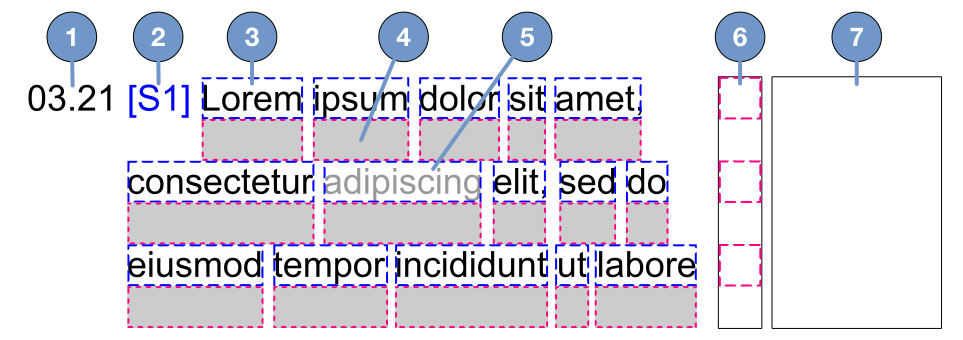
\includegraphics[width=\columnwidth]{figs/paper-interface-diagram}
  \caption[Layout of the paper interface.]{Layout of the paper interface, with timestamps at beginning of each
  paragraph (1), speaker diarization (2), word deletion (3), word selection (4), confidence shading (5), line selection
(6) and a margin for freehand notes (7). Dotted lines indicate hidden active zones for selection (pink) and deletion
(blue).}
  \label{fig:paper-interface-diagram}
\end{figure}

\begin{figure}[p]
  \centering
  \includegraphics[width=\columnwidth]{figs/paper-interface-example-annotations.png}
  \caption{Example of the paper interface system, with freehand annotations that demonstrate its use.}
  \label{fig:paper-interface-example}
\end{figure}

\begin{figure}[p]
  \centering
  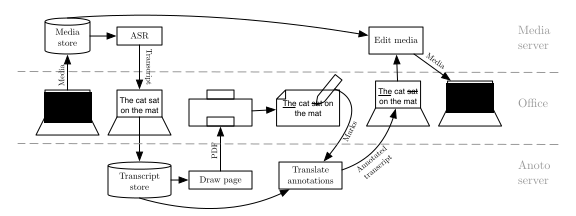
\includegraphics[width=\columnwidth]{figs/uist-sys-diagram}
  \caption{Flow diagram of PaperClip, showing the integration between the paper and screen interfaces, flowing from
  left to right.}
  \label{fig:paper-screen-integration}
\end{figure}


Editing was performed using an Anoto Live Pen 2 digital pen, which tracked and digitally recorded the gestures made on
the transcript.  When the pen was connected to a computer via a USB dock, the gestures were processed and translated by
the Anoto system into edit commands.  We integrated PaperClip with our screen interface (see
Section~\ref{sec:paper-screen-design}) to handle audio import, printing transcripts, viewing/changing edits, viewing
the margin notes and exporting the edits.  A diagram of this integration is shown in
Figure~\ref{fig:paper-screen-integration}.

We supported two export formats --- audio as a WAVE file, or an edit decision list (EDL) for the SADiE or StarTrack
DAWs.  PaperClip also created a PDF document of the transcript that showed the user's annotations, which could be
viewed through the screen interface.

















\subsection{Screen interface}\label{sec:paper-screen-design}

For the screen interface, we updated the system we developed in Chapter~\ref{sec:screen} to implement some of the
changes suggested by our findings.  The original design can be seen in Figure~\ref{fig:interface}
(p.~\pageref{fig:interface}), and the updated design is shown in Figure~\ref{fig:dialogger-interface}.  The original
design used a drag-and-drop system for creating clips from selected text. We replaced this with underlining and
strikethrough gestures to provide better support for large selections, and to align with the design of PaperClip.

\begin{figure}
  \centering
  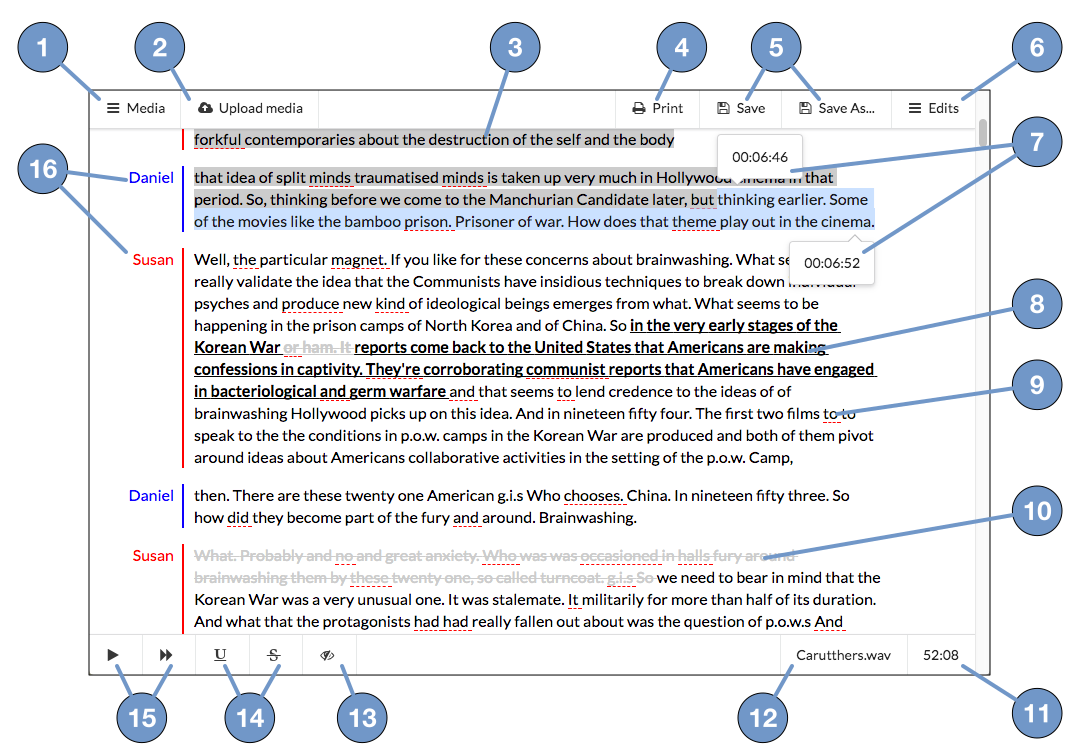
\includegraphics[width=\columnwidth]{figs/discourse-interface-labelled}
  \caption[User interface of the screen-based semantic speech editor.]{User interface of the screen-based semantic
    speech editor, which features 
    media storage (1),
    media upload (2),
    highlight of the current playback position (3),
    printing the transcript (4),
    saving edits and corrections to transcript (5),
    edit storage and export (6),
    displaying timestamps of the current selection (7),
    underlining words (8),
    confidence shading (9),
    strikethrough of words (10),
    display of edited audio duration (11),
    name of current asset (12),
    show/hide strikethrough (13),
    underlining/strike buttons (14),
    playback buttons (15)
  and speaker diarization (16)}
  \label{fig:dialogger-interface}
\end{figure}

We added a double-speed playback feature to allow faster than real-time listening, and a ``save-as'' feature to allow
multiple edits of the same material.  We implemented this by using collapsible sidebars to separate the original
``media'' on the left, from the modified ``edits'' on the right (see Figure~\ref{fig:download-pdf}).  We also included
speaker diarization using a label and line down the side of each paragraph, coloured by gender, and included confidence
shading using a dotted red underline to match the style of word processors.

\begin{figure}
  \centering
  \includegraphics[width=0.4\columnwidth]{figs/discourse-download-pdf.png}
  \caption[Close-up of the edits sidebar of the screen-based semantic speech editor.]{Close-up of the edits sidebar of
  the screen-based semantic speech editor, showing a button to export audio, and a dropdown menu with the option to
download a PDF.}
  \label{fig:download-pdf}
\end{figure}


The screen interface included integrated playback, which allowed the user to listen to and navigate the audio while
they edit. The current playback position was shown in the text and the user could jump to a word by double-clicking it
on the transcript. Any edits made to the transcript were reflected in the audio.  The user could also correct any
mistakes in the transcript by editing the text as they would in a word processor.









\section{Evaluation methodology}\label{sec:paper-method}

The objective of our second study was to discover whether professional radio producers could use PaperClip as part of
their workflow, and to compare how the workflow was affected by PaperClip and our screen interface.  To find out, we
ran a within-subjects qualitative user study in which we tested radio producers editing speech recordings under three
different conditions:

\begin{enumerate}[label=C\arabic*.]
  \item PaperClip digital pen interface
  \item Screen interface
  \item Normal printed transcript
\end{enumerate}

We did not want to test the impact of the transcript itself, but rather the impact of the interface that was used to
interact with the transcript. Therefore, all three conditions used a transcript generated by the same ASR system,
developed by the BBC. Our ASR used the Kaldi toolkit\footnote{\url{http://kaldi-asr.org/}} and was trained on
television recordings.  The normal printed transcript acted as a control. It included speaker labels and timestamps,
but did not use the PaperClip layout or Anoto dot pattern.

We recruited eight radio producers from the current affairs, science and documentaries teams in BBC Radio.
Table~\ref{tab:participants} lists the participants and their self-reported professional experience and the department in
which they work.
Only one of the
participants overlapped with our first study in Section~\ref{sec:paper-requirements}.  As producers are very busy, we
designed our study to take less than a day to complete. Despite this, it took us 12 months to recruit the participants
and collect the data as producers often cancelled or re-arranged due to their demanding role.

\begin{table}[h]
  \centering
  \begin{tabular}{l l l}
      \hline
      \textbf{ID} & \textbf{Experience} & \textbf{Department} \\ %
      \hline
      P1 & 13 years & Current affairs \\%& Medium  \\
      P2 & 16 years & Documentaries   \\%& Low     \\
      P3 & 8 years & Current affairs \\%& High    \\
      P4 & 10 years & Science         \\%& High    \\
      P5 & 18 years & Current affairs \\%& Low     \\
      P6 & 16 years & Current affairs \\%& Medium  \\
      P7 & 28 years & Documentaries   \\%& Medium  \\
      P8 & 20 years & Science         \\%& Low     \\
      \hline
  \end{tabular}
  \caption{Evaluation study participant demographics.}
  \label{tab:participants}
\end{table}







\subsection{Protocol}

The protocol for our study had three stages.

\paragraph{Stage 1: Training}

Firstly, the participant was briefed on the study and asked to sign a consent form.  The participant used a test
recording to perform a scripted series of tasks that used all of the features of each interface.  This allowed them to
use and experience all of the features for themselves. The participant was then given an opportunity to ask questions
and become familiar with each interface until they felt comfortable with using them.

\paragraph{Stage 2: Observation}

The participant completed three editing tasks, each under one of the three conditions (C1, C2 or C3).  The order of
conditions was balanced to avoid carryover effects.  We designed the experiment so that the editing tasks
overlapped with the work the producers already needed to do. This ensured that the tasks were genuine and part of a
real production.  The participant provided three recent speech recordings that they needed to edit so that the content
was fresh in their mind.  We needed to use different recordings for each condition, but we asked the participant to
choose recordings from the same programme to ensure they were as similar as possible.  In Chapter~\ref{sec:screen}, we
found that there was no benefit in using transcripts for short recordings, so each recording was at least 20 mins in
length. 
 
The investigator observed the task, made written notes about their behaviour, and logged the duration of each audio
file and the time taken to edit it, excluding any interruptions.  Items of interest at this stage included editing
workflow, tools used, data generated, usability challenges and problems, navigation and edit actions, time taken to
complete tasks, unexpected reactions and unanticipated usage. During any ``down-time'', we conducted ad hoc, in situ
interviews to clarify the process and any decisions that were made.  The observation took place at the participant's
normal work environment, which in all cases was a desk in an open plan office.  We considered recording the task using
a video camera, but due to the open-plan nature of the offices, there were insurmountable issues with privacy and
information security.

After each task, the participant filled out a questionnaire to measure the usefulness and usability of the interface,
using the Perceived Usefulness scale \citep{Davis1989} and the Software Usability Scale (SUS) \citep{Brooke1996},
respectively.  After completing all three tasks, the participant was asked to select which system they would prefer to
continue using.












\paragraph{Stage 3: Interview}

The investigator conducted a semi-structured interview using the following questions.  The order of questions 2--4 was
adjusted to match the order in which the conditions were presented to the participant.  An audio recording was made of
the interview for later analysis.



{\singlespacing
  \begin{enumerate}
    \item Can you please describe your existing process for editing audio?
    \item What did you like or dislike about the pen-based system?
    \item What did you like or dislike about the screen-based system?
    \item What did you like or dislike about using normal paper?
    \item Overall, which of these systems would you most prefer to continue using, and why?
  \end{enumerate}
}




\subsection{Analysis}

We transcribed the interview recordings and corrected the words manually using the screen interface described in
Section~\ref{sec:paper-screen-design}.  Using
thematic analysis \citep{Braun2006}, the investigator then openly coded the transcripts and observation notes using
\textit{RQDA} \citep{RQDA}, which produced 229 initial codes. The investigator then used \textit{FreeMind} mind-mapping
software to group the codes into categories, and the categories into themes.

The time taken to edit an audio file depends upon its length.  As recommended by \citet{Dewey2014}, we divided the edit
speed of each task by the audio file duration to calculate the ``normalised task completion time''.  Following the
procedures described in \citet{Davis1989,Brooke1996}, we converted the questionnaire data measuring the usefulness and
usability into individual scores between 0 and 100. We used within-subjects one-way ANOVA \citep{Rouanet1970} to test
for differences between the systems in the relative edit time, perceived usefulness and usability (SUS) metrics.  For
the system preference data, we simply report the count of the preferences for each system.





\section{Evaluation results}\label{sec:paper-results}

In this section, we will present the quantitative and qualitative results that emerged from the metrics, observation
notes and interviews in our evaluation study.  The themes and categories that resulted from the analysis of the
interview transcripts and observation notes are shown in Table~\ref{tab:paper-codes}.  We will start by looking at the
metrics and user preferences we gathered, before summarising the comments made by participants in each of the
categories and themes that emerged from the thematic coding process.

\begin{table}[p]
  \centering
  {\small
    \begin{tabular}{l l l} %
      \hline
      \textbf{Theme} & \textbf{Category} & \textbf{\# codes} \\ \hline
      \multirow{8}{*}{Editing}
      & Collaboration & 15 \\ %
      & Annotation & 16 \\ %
      & Location & 11 \\ %
      & Export & 7 \\ %
      & Pen & 35 \\ %
      & Technique & 24 \\ %
      & Decisions & 12 \\ %
      & Interface & 21 \\ \hline %
      \multirow{4}{*}{Transcript}
      & Paper & 15 \\ %
      & Accuracy & 17 \\ %
      & Generation & 10 \\ %
      & Correction & 12 \\ \hline %
      \multirow{3}{*}{Listening}
      & Navigation & 8 \\ %
      & Criteria & 14 \\ %
      & Technique & 12 \\ \hline %

    \end{tabular}
  }
  \caption{Themes, categories and number of codes that resulted from the quantitative analysis of the interviews and
  observations.}
  \label{tab:paper-codes}
\end{table}


\subsection{Metrics}\label{sec:paper-metrics}

\begin{figure}[p]
  \centering
  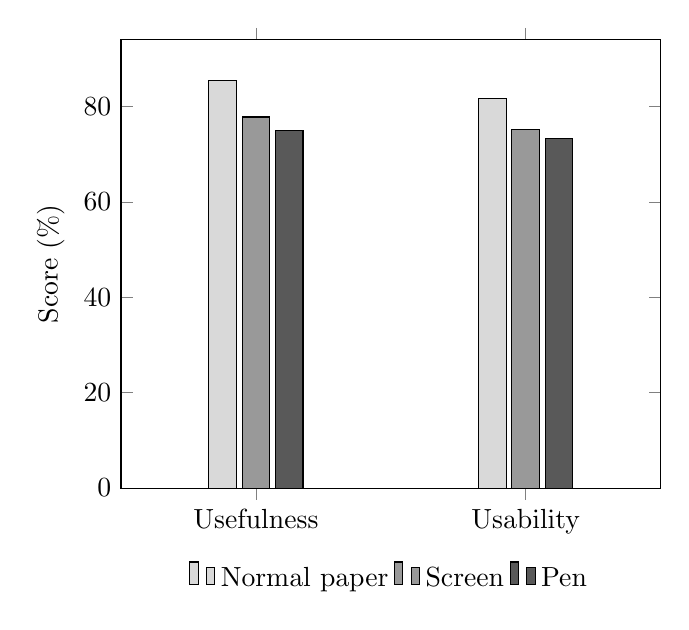
\begin{tikzpicture}
    \begin{axis}[
      ybar,
      ymin=0,
      enlarge x limits=0.5,
      legend style={at={(0.5,-0.15)},anchor=north,legend columns=-1,draw=none},
      ylabel={Score (\%)},
      symbolic x coords={Usefulness, Usability},
      xtick=data,
      ]
      \addplot[fill=black!15] coordinates {(Usefulness,85.42) (Usability,81.67)};
      \addplot[fill=black!40] coordinates {(Usefulness,77.78) (Usability,75.21)};
      \addplot[fill=black!65] coordinates {(Usefulness,75.00) (Usability,73.33)};
      \legend{Normal paper, Screen, Pen}
    \end{axis}
  \end{tikzpicture}
  \caption[Mean average scores for usefulness and usability.]{Mean average scores for usefulness and usability. There
  is no statistically significant difference between the scores.}
  \label{fig:pen-useful-usable}
\end{figure}

When asked which system they would prefer to continue using, four of the eight participants chose PaperClip, two (P3
and P6) chose the screen interface and two (P1 and P4) chose the normal paper transcript.  Although it did not include
any semantic editing functionality, P1 and P4 said they preferred the normal paper transcript as it allowed them to use
their existing workflow and tools, which they found easiest and most comfortable.  This demonstrates that ASR
transcripts themselves are beneficial to radio production.

Figure~\ref{fig:pen-useful-usable} shows the mean average scores of the usefulness and usability of the three systems.
A one-way within-subjects ANOVA showed that there was no statistically significant difference between the systems for
usefulness [$F(2,14)=0.788, p>0.05$], nor usability [$F(2,14)=1.068, p>0.05$].

The SUS metric produces a numeric score between 0 and 100, which can be used to directly compare the usability of
different systems.
The reported SUS scores of systems from other studies can be used to convert our scores into a percentile figure that
shows how they compare to other interfaces in general.  \citet[p.~204]{Sauro2016} proposed translating this percentile
score into a grade between F and A+ to describe the result in human terms.
The grades for our normal paper, screen and pen interfaces were A, B and B--, respectively, which shows that all of the
tools appear to perform well overall.  However, as this technique does not take into account the purpose
of the interfaces, it cannot tell us how usable our interfaces are compared to other semantic speech editors.


For each task, we divided the edit time by the audio duration to calculate the relative edit time.  The screen and
normal paper interfaces had the same mean relative edit time ($\times 0.99$ real-time), but PaperClip was 16\% faster
($\times 0.83$ real-time).  This was surprising, as we expected the screen interface to be faster than both the pen and
normal paper due to its integrated playback feature.  However, a one-way within-subjects ANOVA did not find any
statistically significant difference [$F(2,14) = 0.931, p > 0.05$].

The metrics results show that although half of participants preferred the PaperClip interface and it had the fastest
relative edit time, it was rated least useful and least usable. 
To try to better understand these ratings, we now turn to the interview and observational
data.


























\subsection{Editing}





\subsubsection{Decisions}
Participants P4, P5 and P8 reported that they could make editorial decisions faster and more easily on paper compared
to the screen because of the reduced functionality of the interface, uninterrupted playback of the audio, natural edit
gestures and faster reading speed.  P4 said that the lack of correction features in PaperClip allowed them to
edit faster than the screen, as it didn't interrupt their flow.

\textit{``I liked how it limited my options, [...]
  because with the screen I think what slowed me down
  was the fact that I could be
  [...] simultaneously correcting the transcript and trying to edit the content. [...]
  With the pen, I couldn't, so there's no point stopping. [...]
  I don't think I've ever done an edit that fast, where it was literally real-time.''} (P4)



P2 and P5 reported that they could process the information faster when reading on paper compared to the screen. P5 said
that when using the screen, they would select more than necessary because their decision-making couldn't keep up with
the audio.


\textit{``The [screen] felt too quick and much harder to make a decision. It was like
  `just keep everything', because you don't want to miss something.''} (P5)

P8 said they felt that the digital pen allowed them to be more precise with their edits than with the screen.  Although
the screen is just as precise, the digital pen can be used to start making a selection without knowing the endpoint.
This allows the producer to decide as they listen, which may give a feeling of better control over precision.



\subsubsection{Pen}

P5, P6 and P8 felt that the physicality of the PaperClip interface made it user friendly, intuitive and simple.

\textit{``It feels like you're working analogue, but you're actually working digitally. [...] It's nice to hold a pen
and go on real paper, which has the feel of every day life.''} (P7)

The design of PaperClip forced users to select or delete content by drawing lines within strictly defined zones
that are interpreted literally. P3, P5, P7 and P8 said they did not like that they could not freely draw on the page and were
concerned about potential errors that could be introduced by straying outside of the boundaries.

\textit{``[PaperClip] doesn't have the convenience of paper, which is that there's no real rules [and] you can
write anywhere on the paper.''} (P3)




P3 and P6 said that they did not like that there wasn't any way to undo the edits using PaperClip. P6 suggested
that the lack of undo functionality may force them to be more decisive.

\textit{``It's harder to say `oh no I've changed my mind, I want to go back', so you almost have to be much more
decisive, which maybe is a good discipline.''} (P6)


P2, P3, P5 and P7 were interested in the cost of the pen as they were concerned about losing or breaking a potentially
valuable item.  P3 and P5 noted that other valuable items, like headphones and recorders, are normally shared amongst
producers in a team but that they often disappear or get broken.


\textit{``Pens which are not connected to anything will go missing and get lost.
  [We have a] constant problem with headphones going missing in this department [...]
and the solution is that the headphones are actually bolted to the desks.''} (P3)

Often transcripts can be very long, so printing them requires a large amount of paper. P2 used a long recording
for the experiment that required over 50 sheets of paper, which they said was \textit{``quite wasteful''}.
The Anoto system also requires access to a colour laser printer.
This is not usually a problem in an office environment, but can be an issue when travelling, or when
working from home.







\subsubsection{Collaboration}
Radio producers work with a variety of people including presenters, assistant producers, contributors and
organisations.  P3, P6 and P7 said that transcripts make it easier to collaborate as they create a common reference
point that is easy to share and annotate.

\textit{``The way we're doing it is printing out our transcripts and we can all go `page 15' [...]
there's a common reference, whereas if you're just doing audio it's harder.''} (P6)

The physical nature of paper allows people in the same room to hand around transcripts, point at words and lay pages
out. However, the digital nature of the screen means it can be used for remote collaboration. For example, P6 reported
that they use Google Docs to simultaneously write and edit the script remotely with the presenter.



\textit{``I think of the three, [the screen] has the most potential to be a collaborative thing. [...]
  Maybe if you could have two scripts side by side to have my transcripts with my bits highlighted and the presenters,
with their bits highlighted.''} (P6)



\subsubsection{Location}
P1, P5, P7 and P8 said that they often prefer to work away from the office, such as at home, to help them focus and get
more work done.  P7 and P8 suggested that PaperClip was well-suited for travel, such as during commuting, which
may provide an additional opportunity to be productive in what would otherwise be considered downtime.  Although, P7
pointed out that the screen interface could be used on-the-road with a laptop and noise-cancelling headphones. 


\textit{``With the pen you could do stuff on the train [...]
or on a bus. You could do it anywhere as long as it's not too bumpy.''} (P8)

P5 said they did not enjoy spending too long sitting upright at their
desk, and P7 cited comfort as a factor in where they prefer to work.

\textit{``I would feel more comfortable with a nice digital pen and a sheet of paper sitting on a couch [...]
  You could do it in bed - that would really have your work-life balance sorted, wouldn't it?''} (P7)

\subsubsection{Technique}
P1, P2, P6 and P8 reported that editing was an iterative process. P2 said this was because they are not sure what they
need in the early stages, so they select too much then reduce it later. P8 said that what they select, or how much they
select, depends on what was said in other interviews, and P1 said they often have to go back to re-edit clips in a
different way. 





P1, P6 and P8 reported that all three systems we tested were only suitable for the first iteration, known as a ``rough
edit'', because they were missing two features --- re-ordering and labelling. Re-ordering is used to to see and hear how
different clips from separate interviews would work together, and labelling is used to help the producer navigate,
organise and structure their content. 




P5 used annotations to segment and label the transcript (see Figure~\ref{fig:p5-annotations}), which helped to
structure the material.

\textit{``I was just labelling by summarising a paragraph in about two or three words --- just who is speaking and the
substance of it --- or maybe just putting a cue to say that was a question.''} (P5) 

\begin{figure}[h]
  \centering
  \includegraphics[width=\columnwidth]{figs/print/pen-annotations-p5-cropped-bw.jpg}
  \caption{Annotations made on paper in the margin by P5. The content is segmented using horizontal lines and labels in
  the margin.  The middle segment is marked as not needed using a diagonal line.}
  \label{fig:p5-annotations}
\end{figure}



By capturing this information in a structured way, it could be exported as part of the EDL to guide the producer in
later stages.  P3 suggested that it might be possible to automatically generate labels using the text of a selected
clip.

\textit{``If it was to dump those separate clips in your [system] and name them according to the text, then that would
save twenty minutes suddenly in a single go.''} (P3)


\subsubsection{Annotation}




PaperClip used an underlining gesture to select words, but P1 and P6 both suggested that they would prefer using a
highlighter pen style mark.  This would also mean that the transcript wouldn't have to be double-spaced, but it would
require a system that can distinguish between a strikethrough and highlight.


Participants used different marks to rate the importance of their selections, including stars and asterisks, which we
witnessed previously in Chapter~\ref{sec:screen}. However, both P2 and P6 suggested using colours as a way of marking
up different selections.  This could be used as a rating system, where one colour is considered more important than
other, or as a categorical system for whatever context is appropriate to that producer.

\textit{``Maybe if you had different colours you could mark your first one in red [then]
change colour and underline it a second time.''} (P6)





\subsubsection{Interface}





The lack of integrated audio playback and navigation in the pen interface made it more difficult for participants to
navigate the audio content.  Although participants could use a separate playback device to navigate the audio,
they either had to do this ``blind'', or use the timestamps on the transcript to guide themselves to the desired
position. With the screen interface, participants could use the text to see where they were navigating to, making it
much easier to move around non-linearly.  We observed that when using the pen interface, many participants chose to
edit while listening straight-through, without navigating the audio at all.

The ease of navigation offered by the screen interface may make it better suited to editing recordings where producers
are more reliant on listening to the audio. This could include content with which the producer is less familiar, such
as a recording they were not present at, or a recording from the archive.

\textit{``I think if you're in a rush, and you know roughly what you've got, and it's an interview that's close to
memory, then the pen's really good. I think if you want to get into the guts of the interview, [...] then you're going
to want to work on the screen.''} (P7)

\subsubsection{Export}

Both the screen and pen interfaces that we tested included a feature to export an edit decision list (EDL) to a DAW.
This allowed the participants to integrate with their existing workflow by being able to make changes to their edits
using their existing tools.  P2 and P6 expressed frustration that annotations were not included in the export.

\textit{``Once you have put it into SADiE you have to [label the content] again. It's almost like you've gone forwards
then you have to take half a step back and you lose a bit of momentum.''} (P2)


The other frustration with the export feature was that in the EDL, the selected clips were all pushed together without
any gaps. P3, P5 and P6 said that they would like there to have been gaps between clips, so that it would be more
obvious where the edits are when listening back. Instead of using gaps P5 and P8 moved their selected clips to a
different track in the DAW when editing with the normal printed transcripts. This also allowed them to see where the
clips were located in the original recording.


\subsection{Transcript}

\subsubsection{Paper}

Most participants commented that working with paper had a number of benefits to their workflow.  P2, P5 and P8 said
they found it easier to read from paper than screen.  P1, P2, P6 and P7 said that it was easier on the eye and gave
them a break from working on screen.  P2, P5 and P7 said they enjoyed that paper was a physical, tangible medium which
they could touch.  P1 and P5 commented that using paper transcripts made it easier for them to orientate themselves.


P1 said the paper interface allowed them to think more widely, and P8 reported that they found it easier to remember
the content of the transcript when reading on paper rather than a screen. 




\textit{``I find it easier to read off paper, and easier to remember stuff.''} (P8)

\textit{``It's essential to print [because]
I have to think more widely. What bits am I going to put where? What's my
  structure? Where am I going to put this bit? Mentally, it is easier for me to refer to the [paper] transcript so
that I know where everything is.''} (P1)



\subsubsection{Accuracy}

All of the participants were successfully able to use the ASR transcripts to edit their material as
part of the production of their radio programme, and all reported that the transcripts were sufficiently accurate for
the purpose of editing their content. Similarly to what we found in Chapter~\ref{sec:screen}, the most common
complaints were of reduced accuracy due to heavy accents or background noise, and problems with speaker labelling and
confidence shading. For example, the ASR system would occasionally give a high confidence score to an
incorrect word, or a low confidence score to a correct word, which caused P3 to mistrust the confidence shading.

\textit{``The things it wasn't sure about weren't actually very often the real mistakes.''} (P3)



P6 normally works with perfect transcripts and found that the errors by the ASR system caused them to rely more on
the audio than they normally would, although P7 and P8 said they could use their memory to ignore many of the mistakes
in the transcript.  P8 reported that lower accuracy transcripts caused them to make rougher edits than they would
normally.





\subsubsection{Correction}

We observed that all of the participants chose only to correct errors that impacted on their ability to
read the transcript.  P2, P4 and P6 said that gross inaccuracies in the transcript distracted them, which caused them
to read more slowly and reduced their editing speed.

\textit{``It's good to have the option to sharpen it up as you go along because, obviously, reading back it'll slow
you down if it's completely the wrong word.''} (P2)


We observed that the ASR system would often make repeated mistakes on an unknown word by mistranscribing it
as a variety of words, which made it difficult to fix.  This usually occurred with names of contributors, or words
specific to the topic of the programme.  P3 and P7 asked whether it would be possible to provide custom training to the
ASR system to tailor it for their specific programme.

\textit{``If you're doing a story about AIDS, there's going to be stuff about anti-retrovirals [...]
The ability to teach it some words would be really good.''} (P3)


\subsubsection{Generation}

The participants in this study re-iterated the finding from Chapter~\ref{sec:screen} regarding frustrations with manual
transcription and the benefits of having the transcript automatically generated.
P1 and P3 stated that the ASR element was the largest benefit of the semantic speech editing systems, as it
freed up that time.

\textit{``The transcription thing for me is eighty percent of the advantage.''} (P3)

P7 reported that they already make regular use of a commercial ASR system called
\textit{VoiceBase}\footnote{\url{https://www.voicebase.com/}, accessed 18/01/2018.} to automatically generate
transcripts.  P5 had previously tried a different commercial system called
\textit{Trint}\footnote{\url{https://trint.com/}, accessed 18/01/2018}, but could not continue due to the cost. None of
the other participants reported having used automatic transcripts as part of their existing workflows.





\subsection{Listening}

\subsubsection{Criteria}

All of the participants chose to listen to the audio while editing with the transcripts. They gave four reasons for
doing so: processing information, efficient navigation, judging quality and identifying non-speech sounds.

P1, P4 and P6 reported that listening while editing made it easier for them to process the information that was being
communicated in the interviews.  P1 and P6 said this helped them to find where corrections needed to be made and to find
words that were inaudible or not actually present.  P2 and P8 suggested that the multi-modal input of listening and
reading helped them to understand the content and make edit decisions.

\textit{``I think reading and listening at the same time makes it easier to take that amount of information on. It's
going into two sensory inputs so it's easier.''} (P8)





Although a transcript can tell you what was said, it does not tell you how it was said. This can change the meaning of
the words, and make the difference between an edit that works or not.
One thing the participants were looking out for were any low quality sounds such as ``umm''s and breaths, which are
distracting to listeners and can reduce the intelligibility of the speech.
The ASR process does not attempt to
transcribe ``umm''s, breaths or non-speech sounds. This means that producers must listen to identify these.
P7 and P8 showed an interest in using the transcript to remove these noises.


P1 was interested in hearing the direction of intonation, that is, whether the voice rises or falls in pitch.
The intonation at the end of a clip must match the beginning of the next clip, otherwise it will be
apparent to the listener that the two have been cut from different parts of a recording. Such information is not
visible using the transcript.

\textit{``It could be that [...] the intonation is going up and it won't work as a clip, so I need to hear it.''} (P1)








\subsubsection{Technique}

P4, P6, P7 and P8 all said that they sometimes edit using only the audio itself. When the audio recording 
is short enough that the producer can remember what was said and where, then there is less need for a transcript. P4
put the cut-off threshold as 15--25 minutes.

\textit{``For interviews that are under 15 minutes, I can hold the whole thing in my head. [...] For things
that are over 25 minutes, then that's when [transcripts] start to become useful.''} (P4)

Some programmes focus more on the auditory experience than the words by combining field recordings, sound effects and
music.  In these cases, there may be little benefit in using transcripts at all.

\textit{``If I was making a heavily `actuality-led' programme, I wouldn't bother with those sort of transcripts because
what you want is the sense of the sound, of its audio environment.''} (P7)

P1 and P7 reported that their existing editing workflow often involves re-listening to the material they recorded in
full, \textit{``from beginning to end''} (P1). They reported that this allows them to refresh their memory, and to
start making decisions on what to lose or to keep.
P2 said that they found manual transcription to be a good opportunity to re-listen to material for similar
reasons.
Although removing the requirement to manually transcribe recordings reduces the burden on producers, there is a risk
that it takes away an opportunity to re-listen to material. This may introduce an unintended negative impact in that
edit decisions are based more on the words that are spoken and less on how the programme sounds.

\subsubsection{Navigation}



P2, P4, P5 and P7 spoke of how they used listening in combination with the transcript to efficiently navigate and edit
the audio. They did this by skipping forwards when what they were hearing was not usable, jumping backwards to review
content that had already been listened to, and seeing if the upcoming audio was something of interest.  If it was not,
then they could avoid listening to it altogether, which would save them time.

\textit{``You can glance at the transcript and just see there's a paragraph of stuff that really is not really relevant
[...] and just discount it, whereas with your ears you've got to listen to the whole thing.''} (P5) 

As we saw in Chapter~\ref{sec:screen}, most participants increased the playback speed when listening using the screen
interface or their DAW to skip through material they thought they might not want to use.




\section{Discussion}\label{sec:paper-discussion}

Through our evaluation study, we achieved our aim of understanding how the radio production workflow was affected by
our paper interface, compared to a screen interface. We also gained further insights into how the accuracy of ASR
transcripts affect the editing process, and how listening is used to complement or replace semantic editing.
We discuss each of these topics below.












\subsection{Paper vs screen}


We found that there were no overall preferences between the paper and screen interfaces, but that there were
advantages and disadvantages of both in different uses and circumstances. Influential factors included the complexity
of the edit, familiarity with the audio, accuracy of the transcript, user location and collaboration.  Broadly speaking,
we found that our pen interface was better for making simple edits involving quick decisions, using familiar content
with a high-quality transcript, for producers working away from their desk, or with others in the same room.  By
contrast, we found that our screen interface was better suited to more complicated editing involving complex decisions,
using less familiar content with a lower accuracy transcript, for producers working at their desk, or with other people
remotely.

Participants reported that using paper rather than a screen made it it easier to read transcripts, remember
information, think widely and orientate themselves. This aligns with previous research that has compared reading on
paper to screens \citep{OHara1997,Kurniawan2001,Mangen2013,Singer2017}. These results show that the benefits of
paper-based working can translate to radio production using ASR transcripts.

On average, editing using the pen interface was 16\% faster than using the screen, but this result was not
statistically significant.
However, three of the participants reported that they could edit faster and more easily using the pen interface compared to the
screen.
This may have been partially due to the faster reading speed of paper and the ability to underline while reading or
listening.  Some participants also suggested that the lack of integrated playback and correction features may have
caused them to focus more on the task at hand, rather than being distracted by correction or navigation.

The screen interface included integrated playback and correction, which made it a more powerful tool.  P7 reported that
this made it suitable for more challenging editing tasks or exploring less familiar content, where the producer needs
to be able to listen and navigate efficiently. The integrated listening also made it better for working with less
familiar or lower accuracy transcripts as participants could tolerate the errors by using their memory of what was
said, by listening or by correcting the errors. The screen makes it easier to listen and correct the errors, so is a
better choice for editing less familiar content or lower quality transcript. 


Three participants reported that both interfaces lacked features for labelling or re-ordering material, which meant
that they were only currently suitable for creating a rough edit. This limits the usefulness of semantic editing in the
later stages of production. For the pen interface, handwriting recognition could be used to label a specified region,
or the nearest selected content. Two participants requested that the labels should be included in the exported EDL, so
that they integrate with their existing tools.

Half of the participants reported that they like to work away from their desk or office as it helps them to focus. Pen
and paper is naturally very portable and can be used almost anywhere. As it is does not use a screen, it is smaller,
lighter, easier on the eyes and has a longer battery life. Several participants reported that this makes it more
suitable for travel, and would allow them to work in more comfortable places. However, the requirement to print the
transcripts makes it unsuitable for working ``on the road'', where new material is recorded outside the office. By
using a laptop or tablet device, the screen interface is also portable. The screen has the advantage of
integrated playback and correction, and could be used on the road as it doesn't need a printer.

Producers do not work alone and need to collaborate with others during production. The physical nature of paper made
the digital pen interface suitable for working with others in the same room, as it allowed them to spatially arrange
the pages and refer to the transcript by pointing. However, it is not possible for the pen interface to be used
remotely. The digital nature of the screen interface makes it easy to work with remote collaborators. There is also
potential to extend the screen interface to use operational transformation \citep{Sun2004}, which would allow multiple
users to edit the same content simultaneously.

Our choice of technology for implementing the pen interface introduced some constraints that affected our design.
Users edited the content by underlining or striking text within a set of rectangular boxes. These gestures were
interpreted literally, which created a potential source of errors, and forced the participants to draw carefully. This
design also prevented us from including correction and undo features. The batch-mode operation of the digital pen also
prevented us from including integrated playback.  By overcoming the constraints of our implementation, a pen interface
with integrated listening, correction and undo could allow users to combine the benefits of working with paper with the
full feature-set of the screen interface. However, there is also a risk that adding more features to the pen
interface could introduce distractions, as we saw with the screen interface.

Electronic paper may provide a technical solution that could bypass these constraints. At the time we developed our pen
interface, there were no e-paper devices that supported digital ink interaction, but these will become available in the
near future.  For example, the \textit{reMarkable} tablet\footnote{\url{https://remarkable.com/}} is an e-paper device
that includes a digital ink interface. Although e-paper displays do not seem to currently perform as well as paper for
reading speed, comprehension or eye fatigue \citep{Jeong2012, Daniel2013}, they are likely to improve over time and may
provide a good middle-ground between paper and screen interfaces. 




\subsection{ASR transcripts}



The accuracy of a transcript has a direct effect on the performance and usage of semantic editing tools. We identified
five different areas that were affected by transcript accuracy: correction, reading speed, reliance on listening,
transcript longevity and edit granularity.

Three participants reported that errors in the transcripts slowed down their reading speed, with some errors being more
distracting than others.  Clearly, the more errors that occur, the more likely it is that corrections will be needed.
However, the majority of participants were only interested in correcting errors that were particularly distracting.
None of the participants needed or wanted to fully correct the transcripts, as this is only required if the transcript
needs to be published. Although publication of transcripts is not currently part of the production
workflow, doing so would make the programmes more easily discoverable and searchable.

The ASR system we used often mistranscribed unknown words into a variety of different words, which prevented the use of
search-and-replace.  This usually occurred with words specific to the programme, such as names of contributors or
locations. To avoid this, producers could add unknown words to the dictionary of the ASR system prior to transcription.
By providing additional contextual information, such as the programme topic or number of speakers, the ASR system could
improve the transcript accuracy by using this to better calculate the likelihood of certain words occurring or by
limiting the number of unique speaker segments.

The participants in our study using listening and memory to tolerate errors in the transcript.  Remembering what was
originally said increased the readability of the transcript and reduced the need to replay the audio.  One participant
reported that transcripts are often retained to help producers search through previously recorded material. However, as
the producer's memory fades, the errors in the transcript of previously recorded material become more of a problem, and
the usefulness of the transcript deteriorates over time.

One participant reported that they selected more material than they needed due to the number of errors in the
transcript.  This suggests that the accuracy of the transcript may affect edit granularity.  Selecting too much
material creates more work for the producer at a later stage, as they have to edit their programme down to a
specific time.

Two participants showed an interest in using semantic editing to remove ``umm''s and breaths. The ASR systems we used
were designed to ignore these sort of noises, rather than transcribe them. When they did appear, they were transcribed
into a variety of words, which made it difficult to find and remove them. By explicitly including ``umm''s and breaths
in the ASR training data, these noises could be highlighted in the transcript, which could give users the option to
remove them automatically.


\subsection{Listening}

We found in Chapter~\ref{sec:screen} that listening was an important part of the editing process. Through our study, we
learned more about how and why the participants listened to the audio for semantic speech editing.  Participants gave
three main reasons for listening --- processing information, judging sound quality and identifying non-speech sounds.

Listening allowed participants to hear what the transcript could not tell them, such as identifying mistakes or
omissions in the transcript, finding where there are environmental sounds and working out whether the quality of the
speech is sufficiently good for inclusion in their programme.  Two participants said that simultaneously reading and
listening made it easier to process the information in the speech, making the edit process more efficient. This falls
in line with previous findings that providing transcripts allows users to process voicemail messages more efficiently
\citep{Whittaker2002}, and improves the comprehension of time-compressed audio \citep{Vemuri2004}.

Half of the participants reported that they sometimes edit audio without a transcript, as they can remember most of
what was said, and when it was said, for audio recordings less than 15--25 minutes long.  For some programmes that
focus on the auditory experience, editorial decisions will be led by the quality of the sound rather than what was
said. In these cases, the cost and overhead of generating a transcript may not be worthwhile, however, it is unclear
exactly where this threshold lies.

Two participants reported that they like to re-listen to their recordings in full to refresh their memory and start
making decisions on what to use for their programme.  Another participant suggested that the current process of manual
transcription gave them an opportunity to re-listen.  Re-listening in full adds overhead to the editing process, but
some participants considered it to be a worthwhile process.  The introduction of ASR transcription removes this
opportunity. There is a risk that semantic editing may cause producers to base their decisions on transcripts rather
than audio, which may affect the quality of the programme.

Listening is an important part of editing, but it is a time-consuming process. This could be reduced by using time
compression techniques to increase the playback speed, as discussed in Section~\ref{sec:background-time-compression},
or using sound event detection to identify and label regions of environmental noise \citep{Duan2014,Kroos2017}.
Including this information in the transcript could help producers identify sounds they do or do not want.  Producers
may also benefit from tools that help them see which edits would work or not.  For example, a graphical representation
of the intonation of speech may help producers identify whether editing two pieces of speech together would sound
acceptable.

\section{Conclusion}\label{sec:paper-conclusion}
We presented the results of a contextual user study of semantic speech editing in professional radio production that
compared a digital pen interface to a screen-based interface.  We found that the pen and screen interfaces both work
well, but that each is better in different situations.

The benefits of reading from paper and the simplicity of the pen interface made it better for fast, simple editing with
familiar audio and accurate transcripts.  The integrated listening and correction features of the screen interface made
it better for more complex editing with less familiar audio and less accurate transcripts.  Unlike the pen, the screen
interface is capable of remote collaboration, but the pen interface may work better when working with others
face-to-face.  The digital pen provides greater flexibility for working away from the desk, but its dependence on
printing makes it difficult to work on the road.  The lack of re-ordering and labelling features in both systems
prevented them from being used beyond rough edit stage.

The accuracy of transcripts is crucial to success of both systems. Lower accuracy transcripts appear to result in more
correction, slower reading speed, more reliance on listening, a shorter transcript ``shelf-life'' and selecting more
audio than necessary. The accuracy could be improved by using programme-specific information in the ASR process.
Listening is an important part of the editing process, with some producers choosing to re-listen to recordings in full.
Listening is used to process information, judge quality and identify non-speech sounds. Transcripts may not be needed
for short recordings or where the auditory experience, rather than the specific speech content, is particularly
important.

